\documentclass{article}
	\usepackage{geometry}
	\geometry{left=2.0cm,right=2.0cm}
	\usepackage{graphicx}
	\usepackage{url}

	\begin{document}
		\begin{center}\textbf{Bo Zhang\\01063214\\}
		\end{center}
		\noindent
		\textbf{Task 1: }Download the 1000 URIs from assignment \#2. Use a tool to remove (most of) the HTML markup.\\\\
		\textbf{Algorithm: }\\
		\indent1. Open the links file ``links.txt''.\\
		\indent2. Reset the output file index.\\
		\indent3. For every link, set the corresponding output file name with the index.\\
		\indent4. Check if the output file exists. If not, try to open the link and write the content to the output file.\\
		\indent5. If there is something wrong, save the link to another file ``missingLinks.txt''.	\\
		\indent6. Move the output file index.\\
		\indent7. Open and read the html files 1 by 1.\\
		\indent8. Remove the HTML markup and save it to corresponding TXT output file. Use the script from \url{http://stackoverflow.com/questions/1936466/beautifulsoup-grab-visible-webpage-text} to remove the HTML markup.\\\\
		\textbf{Source code:}
		\begin{list}{}
			\item download\_HTML.py
			\item process\_HTML.py
		\end{list}
		\noindent
		\\\textbf{Results:}
		\begin{list}{}
			\item folder: htmls
			\item folder: htmls\_processed
		\end{list}
		\indent\\
		\indent In the 1000 original links, there are 18 links dead and 2 mp3 links. Therefore, there are 982 files in the ``htmls'' folder and 980 files in the ``html\_processed'' folder.\\
		\noindent
		\\\textbf{Note:}\\
		\indent Sometimes there are some live URIs unable to be opened tentatively. So it is necessary to check the links in ``missingLinks.txt'' to find out if they are all dead links. Therefore, the script might need to be run several times until all the links in ``missingLinks.txt'' are dead links.\\
		\textbf{\\\\Task 2:}\\
		\indent Choose a query term that is not a stop word and not HTML markup from step 1 that matches at least 10 documents. If the term is present in more than 10 documents, choose any 10 from your list.\\
		\indent As per the example in the week 5 slides, compute TFIDF values for the term in each of the 10 documents and create a table with the TF, IDF, and TFIDF values, as well as the corresponding URIs. The URIs will be ranked in decreasing order by TFIDF values.\\\\
		\textbf{Algorithm:}\\
		\indent1. Open and read the TXT files 1 by 1 until 10 suitable TXT file have been found.\\
		\indent2. Split the content of the TXT file into words.\\
		\indent3. Check the words 1 by 1 and count the number of given term.\\
		\indent4. Compute TF, IDF, TFIDF and add all of the content needed to the output table list.\\
		\indent5. Sort the output list.\\
		\indent6. Print the output table.
		\begin{list}{\textbf{Source code:}}
			\item compute\_TFIDF.py
		\end{list}
		\noindent
		\\\textbf{Results:}
		\begin{figure}[h]
			\centering 
			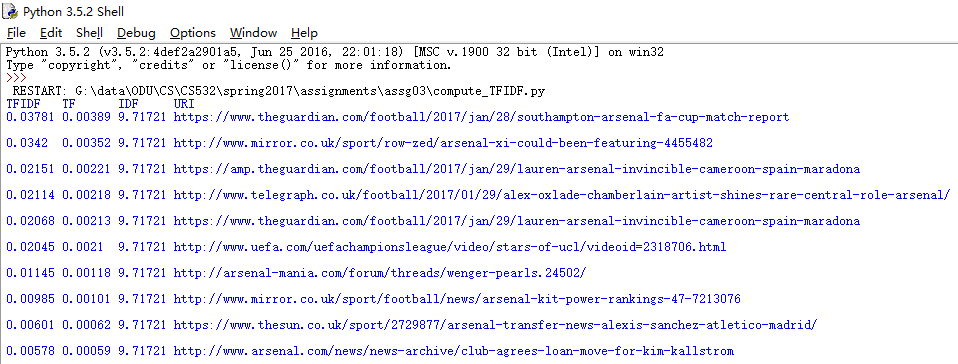
\includegraphics[width=1\textwidth]{TFIDF.png}
			\label{fig:TFIDF} 
		\end{figure}

		\noindent\textbf{Note: }The total pages in google is about 46.8 billion and the pages with term in google is about 55.9 million.
		\begin{figure}[h]
			\centering
			\begin{minipage}{.5\textwidth}
				\centering
				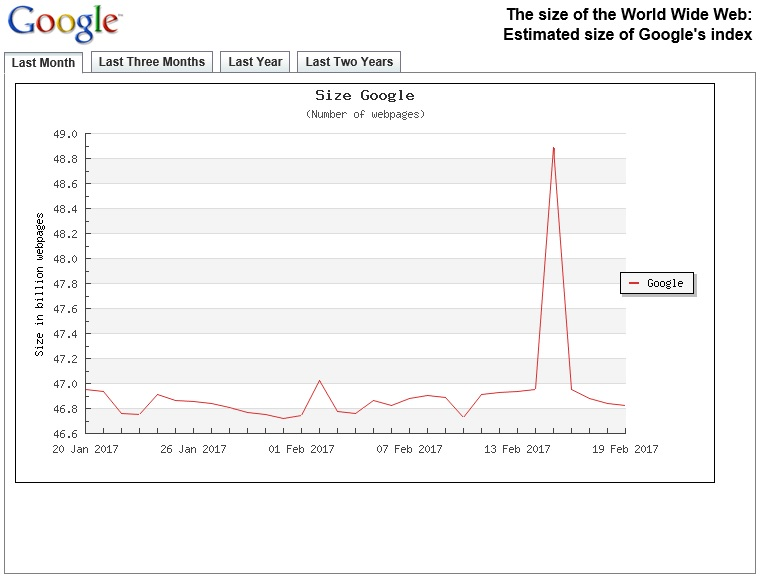
\includegraphics[width=1\linewidth]{googleSize.jpg}
				\label{fig:google size}
			\end{minipage}%
			\begin{minipage}{.5\textwidth}
				\centering 
				
\includegraphics[width=1\linewidth]{wengerGoogle.jpg}
				\label{fig:wenger google}
			\end{minipage}
		\end{figure}

		\noindent
		\textbf{Task 3: }Now rank the same 10 URIs from question \#2, but this time by their PageRank. Normalize the
values they give you to be from 0 to 1.0. Create a table similar to Table 1. Briefly compare and contrast the rankings produced in questions 2 and 3.\\\\
		\noindent
		\textbf{Results:}
		\begin{figure}[h]
			\centering 
			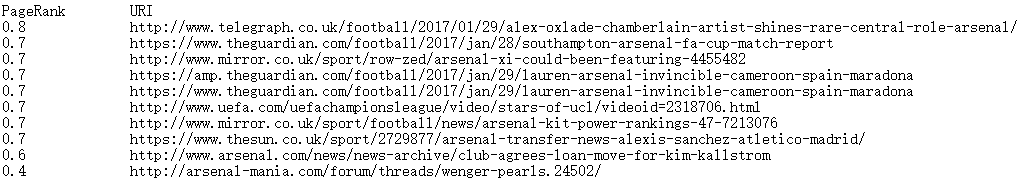
\includegraphics[width=1\textwidth]{PageRank.png}
			\label{fig:PageRank} 
		\end{figure}

		\noindent\textbf{Analysis:}\\
		\indent According to TFIDF, the difference between the 10 links is obvious. The maximum is 6.6 times of the minimum. But according to the PageRank, the difference between the 10 links is very little. Most of the links are 0.7 and the difference between the highest and lowest is only 0.8 v.s. 0.4. For these 2 links, the one with PageRank 0.8 only gets the 4th highest TFIDF and the one with PageRank 0.4 is still the 7th of TFIDF.\\\\\\
		\textbf{Task 4: }Compute the Kendall Tau\_b score for both lists. Report both the Tau value and the ``p'' value.
		\begin{list}{\textbf{R code:}}
			\item Q4\&5.R
		\end{list}
		\noindent\\\textbf{Results:}
		\begin{tabbing}
			\indent\textbf{Correlation Tau}\hspace*{50bp}\=\textbf{P-value}\\
			\indent0.3651484\>0.1815
		\end{tabbing}
		\noindent\textbf{Analysis:}\\
		\indent Due to the p-value, the correlation is not significant enough (just about the possibility of 82\% that the correlation exists). And the coefficient itself is weak too (less than 0.5). Therefore the TFIDF and PageRank of these links have little correlation.\\\\\\
		\textbf{Task 5: }Compute a ranking for the 10 URIs from Q2 using Alexa information. Compute the correlation for all pairs of combinations for TFIDF, PR, and Alexa.
		\begin{list}{\textbf{R code:}}
			\item Q4\&5.R
		\end{list}
		\noindent\\\textbf{Results:}
		\begin{tabbing}
			\indent\textbf{Variables}\hspace*{80bp}\=\textbf{Correlation Tau}\hspace*{50bp}\=\textbf{P-value}\\
			\indent alexa \& PageRank \>-0.573819 \>0.04162\\
			\indent alexa \& TFIDF \>-0.5354632 \>0.03602
		\end{tabbing}
		\noindent\textbf{Analysis:}\\
		\indent Due to the p-values, either the correlation between alexa \& PageRank or alexa \& TFIDF is significant enough (both of the possibilities are more than 95\%). And the absolute values of the coefficients are more than 0.5. Since the coefficients are negative, either the alexa \& TFIDF or alexa \& PageRank of these links have negative correlation, which means the higher alexa score a link has, the lower TFIDF or PageRank it has. Because the nature of alexa score is the lower the better, it is in accordance with TFIDF and PageRank.\\\\\\
		\textbf{Task 6: }Give an in-depth analysis, complete with examples, graphs, and all other pertinent argumentation for Kristen Stewart's (of ``Twilight'' fame) Erdos-Bacon number.\\\\
		\indent A person's Erdos-Bacon number is the sum of one's Erdos number and one's Bacon number. And Kristen Stewart's Bacon number is 2.
		\begin{figure}[h]
			\centering 
			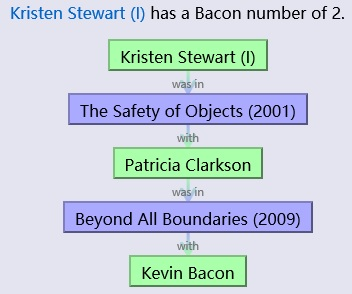
\includegraphics[width=0.4\textwidth]{BaconNumber.png}
			\label{fig:Bacon Number}
		\end{figure}

		For her Erdos number, she has a Donovan Hare Number of 2 and Donovan Hare has an Erdos number of 2. Therefore,  Kristen Stewart has an Erdos number of 4 and her Erdos-Bacon number = 4 + 2 = 6.
		\begin{figure}[h]
			\centering
			\begin{minipage}{.4\textwidth}
				\centering
				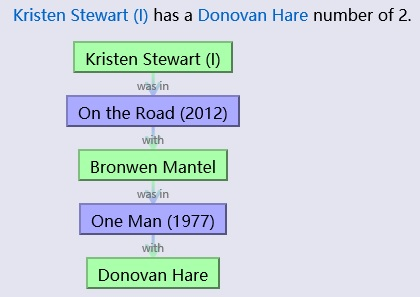
\includegraphics[width=1\linewidth]{DonovanHareNumber.png}
				\label{fig:Donovan Hare Number}
			\end{minipage}%
			\begin{minipage}{.6\textwidth}
				\centering 
				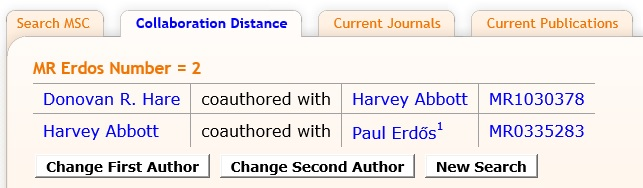
\includegraphics[width=1\linewidth]{ErdosNumber.png}
				\label{fig:Erdos Number}
			\end{minipage}
		\end{figure}

		\textbf{Task 7: }Build a simple inverted file for all the words from your 1000 URIs. Upload the entire file to github and discuss an interesting portion of the file in your report.\\\\
		\textbf{Algorithm:}\\
		\indent1. Set 2 lists for the word index(word and its number).\\
		\indent2. Open and read the TXT files 1 by 1.\\
		\indent3. Split the content of the TXT file into words.\\
		\indent4. Check the words 1 by 1 and compare with the words in the word index.\\
		\indent5. If the word is in the word index, update its number; if not, add it to the word index.\\
		\indent6. Merge the 2 lists into 1 single word index list.\\
		\indent7. Sort the word index list.\\
		\indent8. Output the word index list into the inverted file ``inverted file.txt''.
		\begin{list}{\textbf{Source code:}}
			\item inverted\_file.py
		\end{list}
		\begin{list}{\textbf{R code:}}
			\item Q7.R
		\end{list}	
		\noindent\\\textbf{Results:}
		\begin{list}{}
			\item inverted file.txt
			\item inverted file.csv
		\end{list}
		\noindent\\\textbf{Analysis:}\\
		\indent The top word is ``the''(according to the number) and the top nonstop word is ``arsenal''(because I got these links by searching ``arsenal''). But it is interesting that its number is even more than some stop words such as ``on'', ``for'', ``is'' and ``with'', which may imply that these stop words are less likely to be stop words. The second place of nonstop word is taken by ``news'', which may imply that people tend to tweet news.\\
		\indent And for the frequencies of these words, most of the words occurs less than 32 times and few words occurs more than 1024 times. And the more the frequency is, the less the words are.
		\begin{figure}[h]
			\centering 
			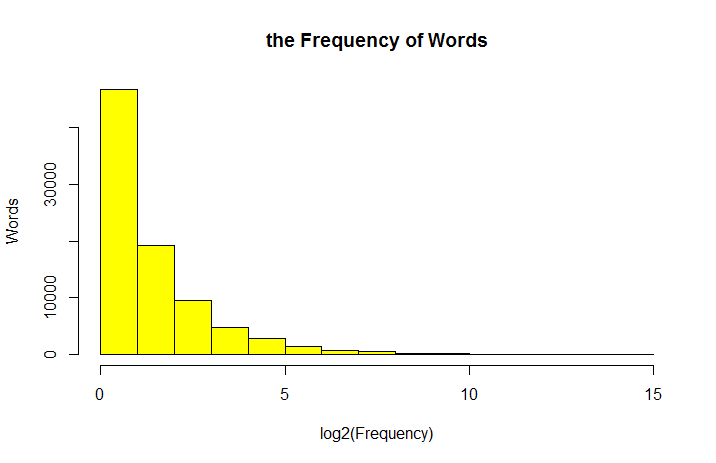
\includegraphics[width=0.65\textwidth]{frequencyOfWords.png}
			\label{fig:frequency of words}
		\end{figure}
	\end{document}